\documentclass[aspectratio=169]{beamer}
\usetheme{Madrid}
\usecolortheme{default}
\usepackage[utf8]{inputenc}
\usepackage{graphicx}
\usepackage{booktabs}
\usepackage{amsmath}
\usepackage{natbib}
\usepackage{hyperref}
\usepackage{xcolor}
\usepackage{caption}
\usepackage{listings}
\usepackage{array}
\usepackage{tikz}
\usepackage{tcolorbox}
\usetikzlibrary{shapes,arrows,positioning}

% Custom colors
\definecolor{hlablue}{RGB}{0,102,204}
\definecolor{hlagray}{RGB}{90,90,90}
\definecolor{managementcolor}{RGB}{0,128,0}    % Green for management
\definecolor{clinicalcolor}{RGB}{128,0,0}      % Red for clinical
\definecolor{bioinfocolor}{RGB}{0,0,128}       % Blue for bioinformatics

% Title formatting
\setbeamercolor{title}{fg=hlablue}
\setbeamercolor{frametitle}{fg=hlablue}

% Bibliography style
\bibliographystyle{apalike}

% Custom commands for audience targeting
\newcommand{\formanagement}[1]{\textcolor{managementcolor}{\textbf{Mgmt:} #1}}
\newcommand{\forclinical}[1]{\textcolor{clinicalcolor}{\textbf{Clinical:} #1}}
\newcommand{\forbioinformatics}[1]{\textcolor{bioinfocolor}{\textbf{Tech:} #1}}
\newcommand{\keytakeaway}[1]{\vspace{0.3cm}\begin{tcolorbox}[colback=yellow!10,colframe=yellow!50!black,title=Key Takeaway]\small #1\end{tcolorbox}}

% Footer
\setbeamertemplate{footline}{
  \leavevmode%
  \hbox{%
  \begin{beamercolorbox}[wd=.25\paperwidth,ht=2.25ex,dp=1ex,center]{author in head/foot}%
    \usebeamerfont{author in head/foot}\insertshortauthor
  \end{beamercolorbox}%
  \begin{beamercolorbox}[wd=.5\paperwidth,ht=2.25ex,dp=1ex,center]{title in head/foot}%
    \usebeamerfont{title in head/foot}\insertshorttitle
  \end{beamercolorbox}%
  \begin{beamercolorbox}[wd=.25\paperwidth,ht=2.25ex,dp=1ex,right]{date in head/foot}%
    \usebeamerfont{date in head/foot}\insertshortdate{}\hspace*{2em}
    \insertframenumber{} / \inserttotalframenumber\hspace*{2ex} 
  \end{beamercolorbox}}%
  \vskip0pt%
}

% Title information
\title[HLA-ProtBERT]{HLA-ProtBERT: AI-Powered HLA Analysis}
\author{NMDP Research Team}
\institute{National Marrow Donor Program}
\date{March 2025}

\begin{document}

% Title slide
\begin{frame}
  \titlepage
\end{frame}

% Executive Summary slide
\begin{frame}{In Brief}
  \begin{columns}
    \begin{column}{0.6\textwidth}
      \begin{itemize}
        \item AI model (ProtBERT) for HLA protein analysis
        \item Captures functional relationships traditional methods miss
        \item Analyzed 17,109 Class I alleles in 81.57 seconds
        \item Reveals biological patterns matching HLA classification
      \end{itemize}
    \end{column}
    \begin{column}{0.4\textwidth}
      \begin{tcolorbox}[colback=hlablue!5,colframe=hlablue]
      \textbf{Benefits}
      \begin{itemize}\small
        \item \formanagement{Efficient analysis pipeline}
        \item \forclinical{Better matching insights}
        \item \forbioinformatics{Novel functional view}
      \end{itemize}
      \end{tcolorbox}
    \end{column}
  \end{columns}
\end{frame}

% Outline slide
\begin{frame}{Overview}
  \begin{columns}
    \begin{column}{0.6\textwidth}
      \begin{enumerate}
        \item HLA Analysis Challenge
        \item AI-Based Approach
        \item Key Findings
        \item Applications
      \end{enumerate}
    \end{column}
    \begin{column}{0.4\textwidth}
      \begin{tcolorbox}[colback=gray!5,colframe=gray!40]
      Content for:
      \begin{itemize}\small
        \item \textcolor{managementcolor}{Management}
        \item \textcolor{clinicalcolor}{Clinical Scientists}
        \item \textcolor{bioinfocolor}{Bioinformaticians}
      \end{itemize}
      \end{tcolorbox}
    \end{column}
  \end{columns}
\end{frame}

\section{The Challenge}

\begin{frame}{HLA Complexity}
  \begin{columns}
    \begin{column}{0.6\textwidth}
      \begin{itemize}
        \item Thousands of alleles with critical immune function
        \item Sequence similarity is not equivalent to functional similarity
        \item Growing database makes manual analysis impossible
      \end{itemize}
    \end{column}
    \begin{column}{0.4\textwidth}
      \begin{tcolorbox}[colback=gray!5,colframe=gray!40]
      \forclinical{Better transplant matching}
      
      \formanagement{Efficiency gains}
      
      \forbioinformatics{Novel computational approach}
      \end{tcolorbox}
    \end{column}
  \end{columns}
  
  \keytakeaway{HLA complexity requires advanced methods beyond simple sequence comparison.}
\end{frame}

\section{AI Approach}

\begin{frame}{ProtBERT: AI for Proteins}
  \begin{columns}
    \begin{column}{0.6\textwidth}
      \begin{itemize}
        \item AI model trained on 106+ million proteins
        \item Pre-trained for protein language understanding
        \item Captures functional/structural properties
        \item 16M parameters vs. billions in larger models
      \end{itemize}
    \end{column}
    \begin{column}{0.4\textwidth}
      \begin{tcolorbox}[colback=gray!5,colframe=gray!40]
      \forclinical{Finds functionally similar HLAs}
      
      \formanagement{Leverages existing AI advances}
      
      \forbioinformatics{Transfer learning from vast protein data}
      \end{tcolorbox}
    \end{column}
  \end{columns}
  
  \keytakeaway{ProtBERT understands protein "language" beyond simple sequence similarity.}
\end{frame}

\begin{frame}{How It Works}
  \begin{center}
    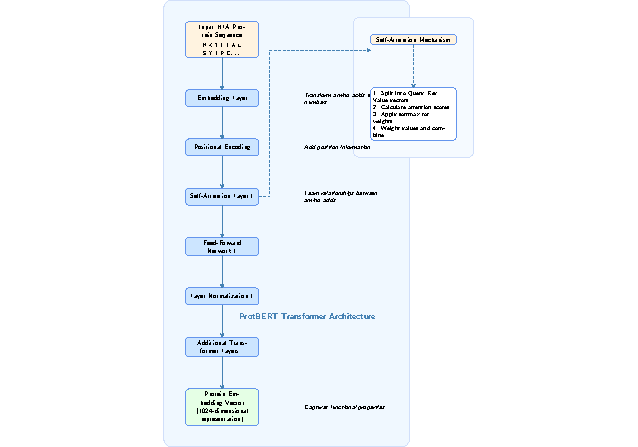
\includegraphics[width=0.60\textwidth]{transformer_diagram.pdf}
  \end{center}

  \begin{itemize}\small
    \item Processes HLA sequence while considering all amino acid relationships
    \item Multiple layers extract increasingly complex patterns
    \item Output: mathematical vector capturing protein properties
  \end{itemize}
\end{frame}

\begin{frame}{From Complex to Simple}
  \begin{center}
    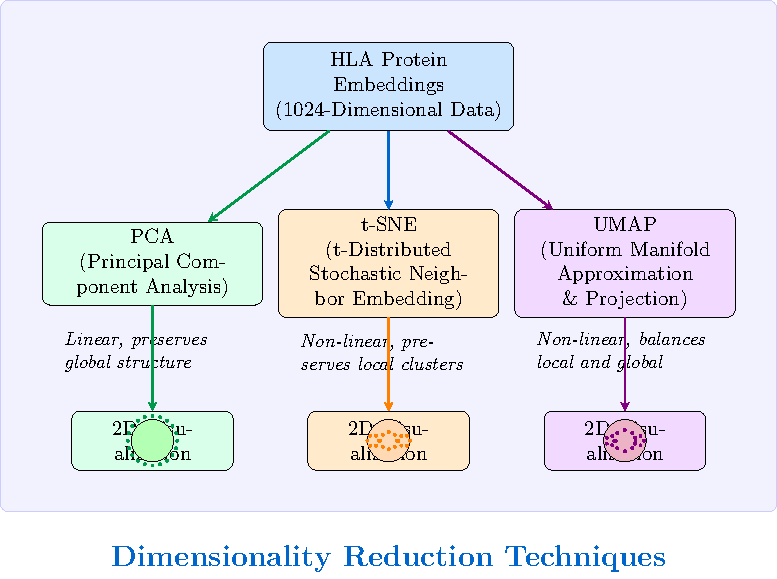
\includegraphics[width=0.5\textwidth]{dim_reduction_diagram.pdf}
  \end{center}

  \begin{columns}
    \begin{column}{0.33\textwidth}\centering\small
      \textbf{PCA}\\
      Global overview
    \end{column}
    \begin{column}{0.33\textwidth}\centering\small
      \textbf{t-SNE}\\
      Local clusters
    \end{column}
    \begin{column}{0.33\textwidth}\centering\small
      \textbf{UMAP}\\
      Balanced view
    \end{column}
  \end{columns}
\end{frame}

\section{Results}

\begin{frame}{Analysis Overview}
  \begin{columns}
    \begin{column}{0.6\textwidth}
      \begin{itemize}
        \item 17,109 Class I alleles analyzed:
          \begin{itemize}\small
            \item 5,432 HLA-A
            \item 6,526 HLA-B
            \item 5,151 HLA-C
          \end{itemize}
        \item Total processing: 81.57 sec (0.005 sec/allele)
        \item Clear clustering by functional groups
      \end{itemize}
    \end{column}
    \begin{column}{0.4\textwidth}
      \begin{tcolorbox}[colback=gray!5,colframe=gray!40]
      \forclinical{Reveals functional similarities}
      
      \formanagement{Demonstrates efficiency at scale}
      
      \forbioinformatics{Effective protein embedding}
      \end{tcolorbox}
    \end{column}
  \end{columns}
\end{frame}

\begin{frame}{HLA-A Visualization}
  \begin{center}
    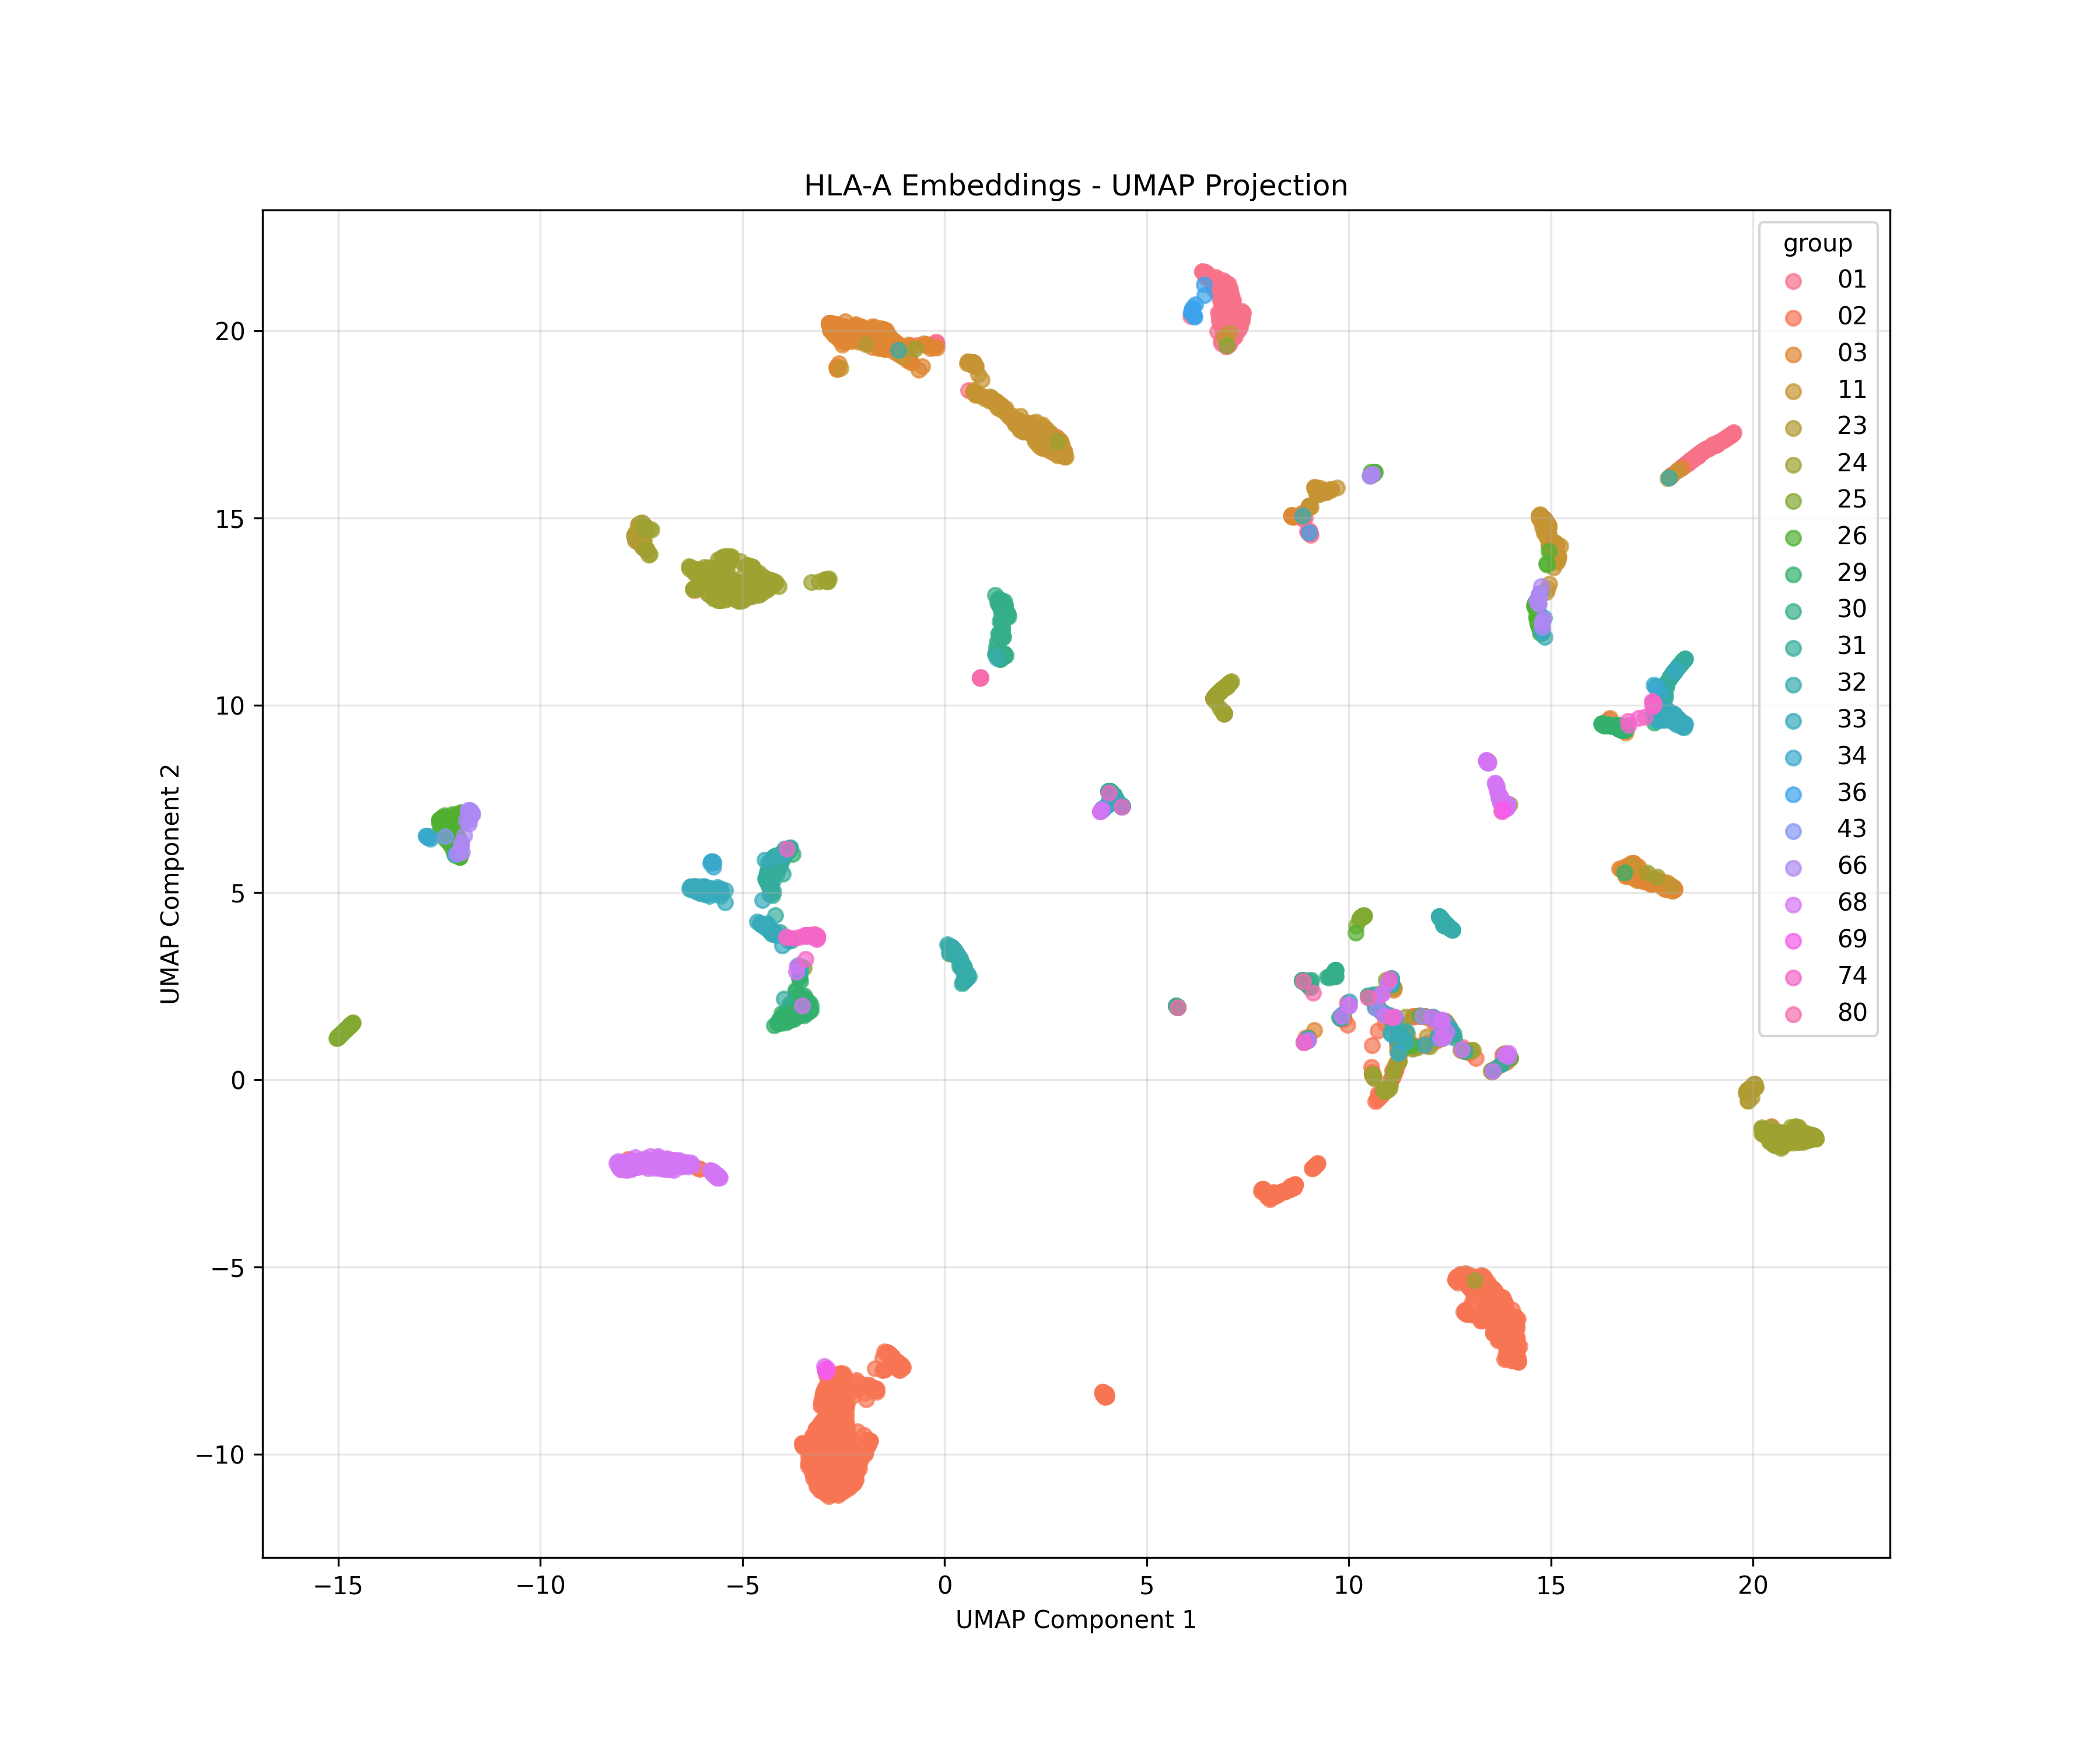
\includegraphics[width=0.5\textwidth]{data/analysis/locus_embeddings/class1/plots/hla_A_umap.png}
  \end{center}
  
  \begin{itemize}\small
    \item Clear separation between major allele families
    \item A*01, A*02, A*03 groups form discrete clusters
    \item May identify unexpected cross-reactive groups
  \end{itemize}
\end{frame}

\begin{frame}{HLA-A: Multiple Perspectives}
  \begin{figure}
    \centering
    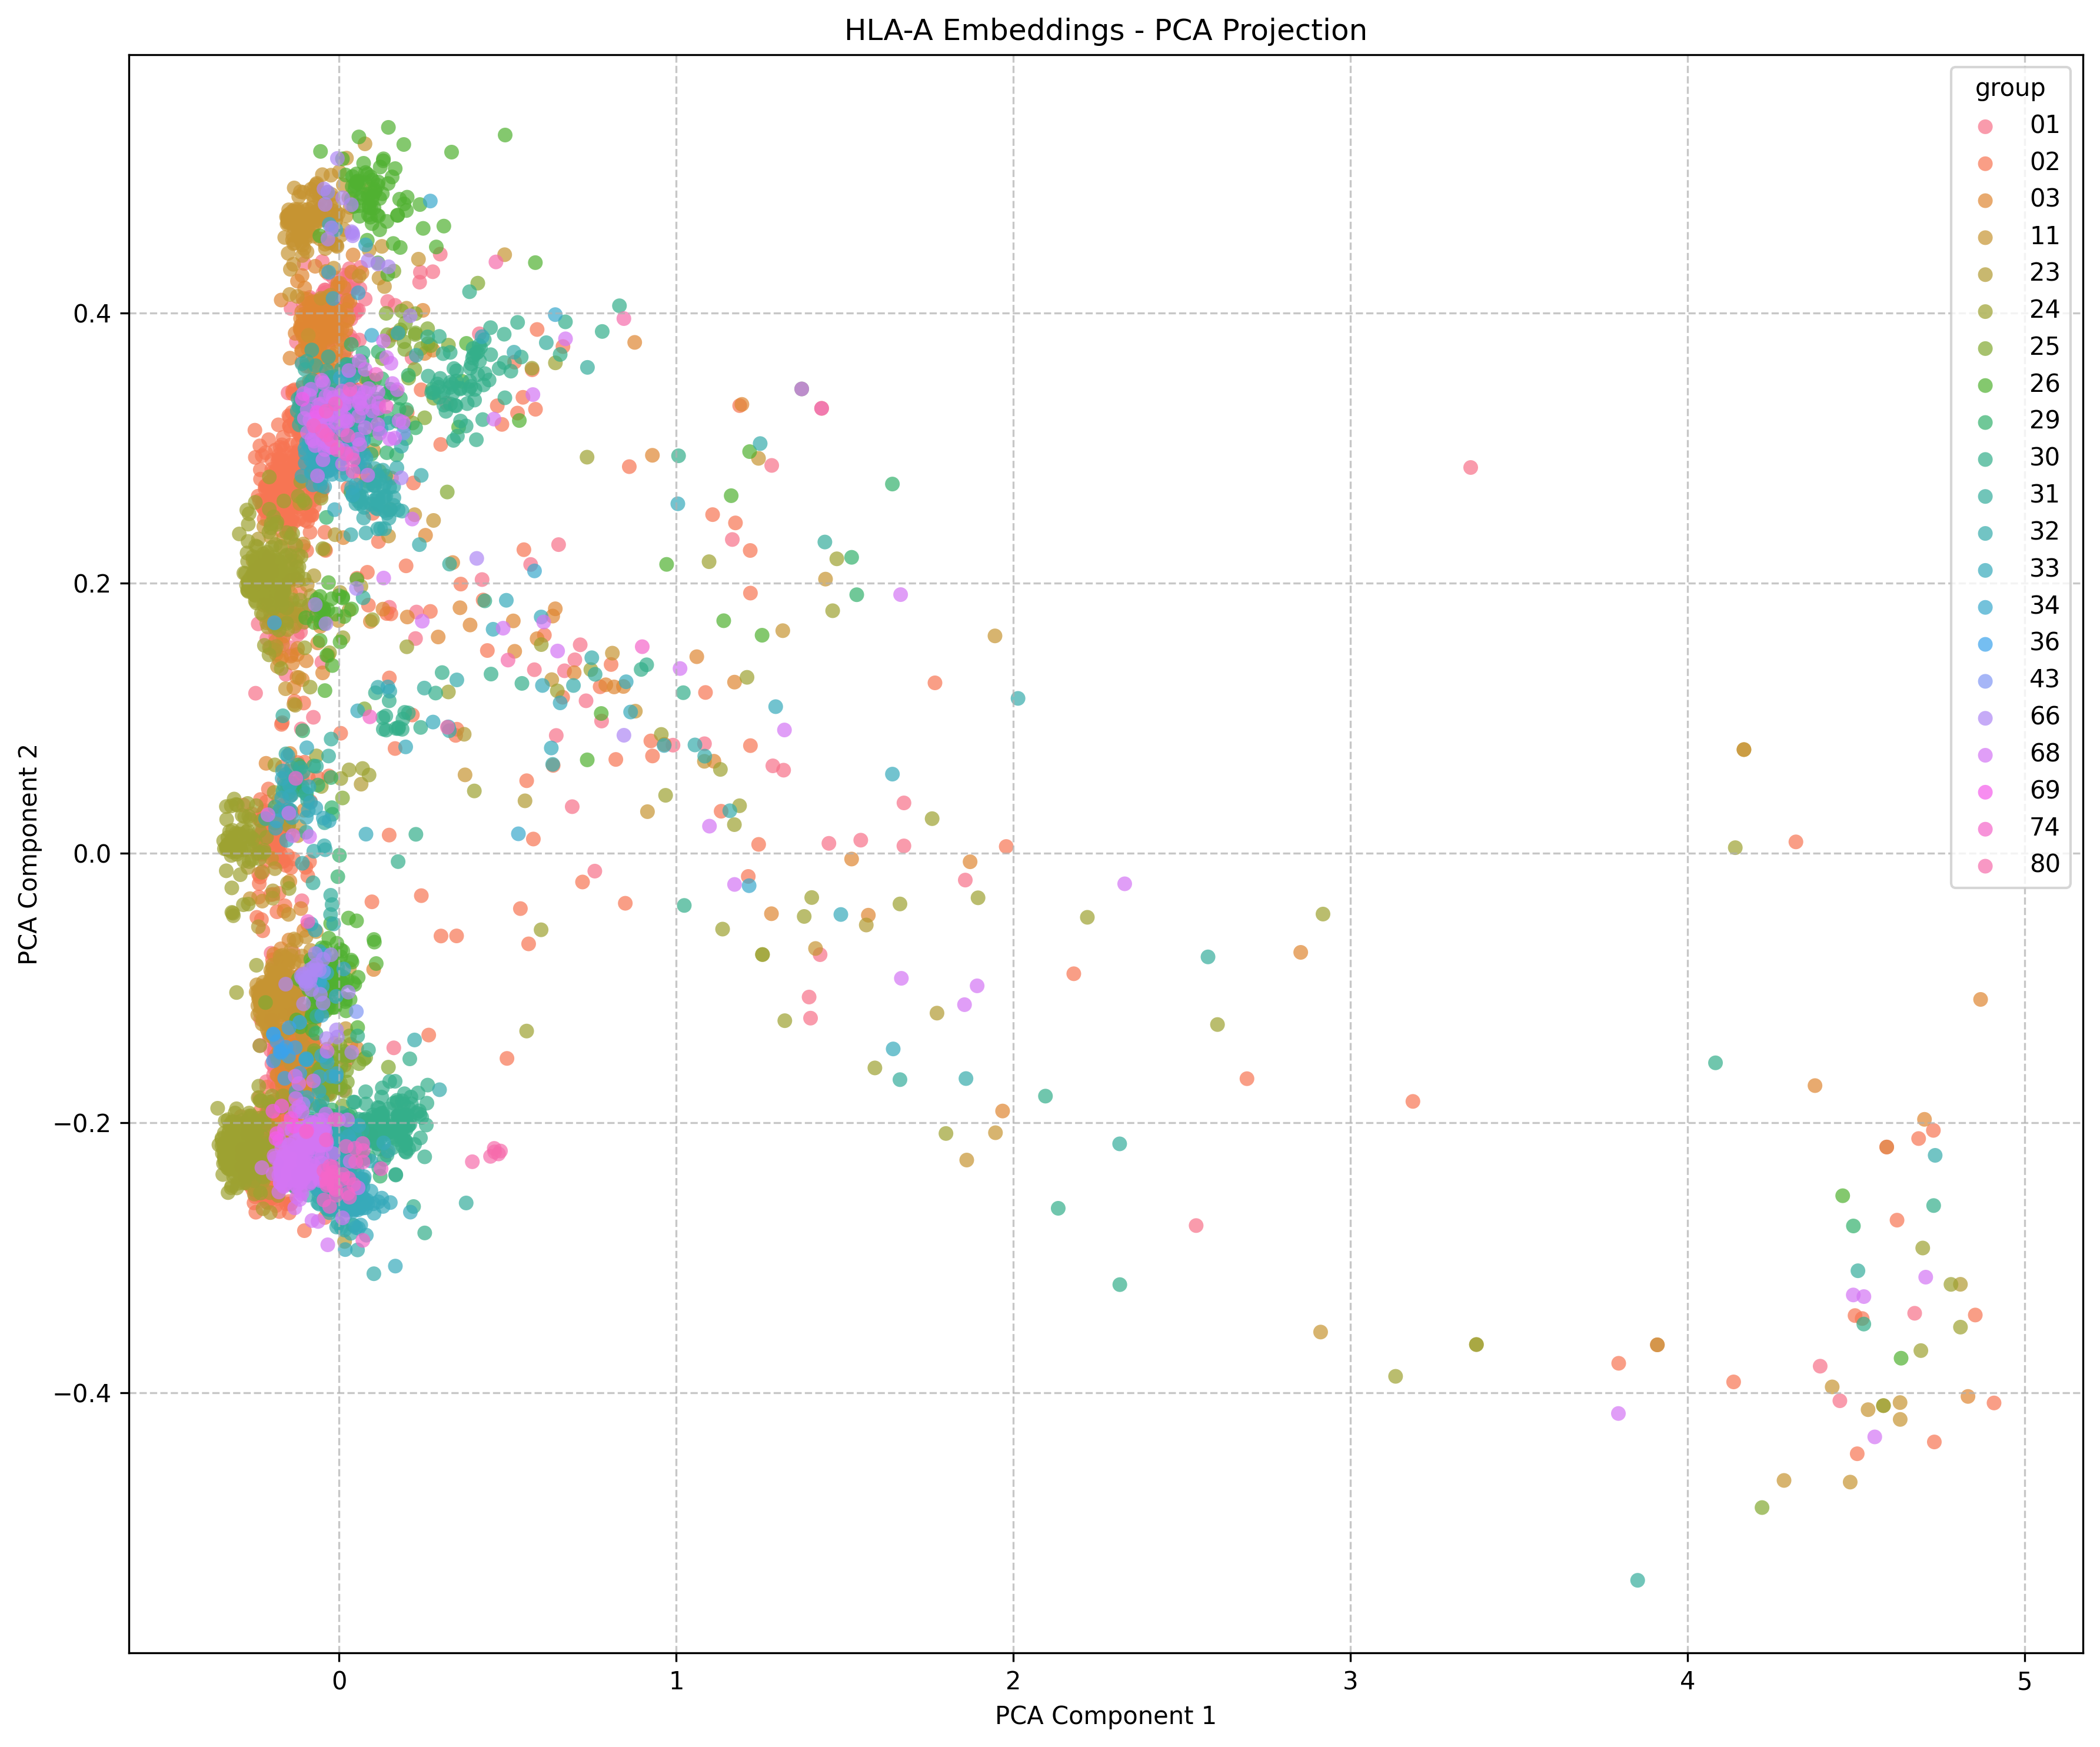
\includegraphics[width=0.32\textwidth]{data/analysis/locus_embeddings/class1/plots/hla_A_pca.png}
    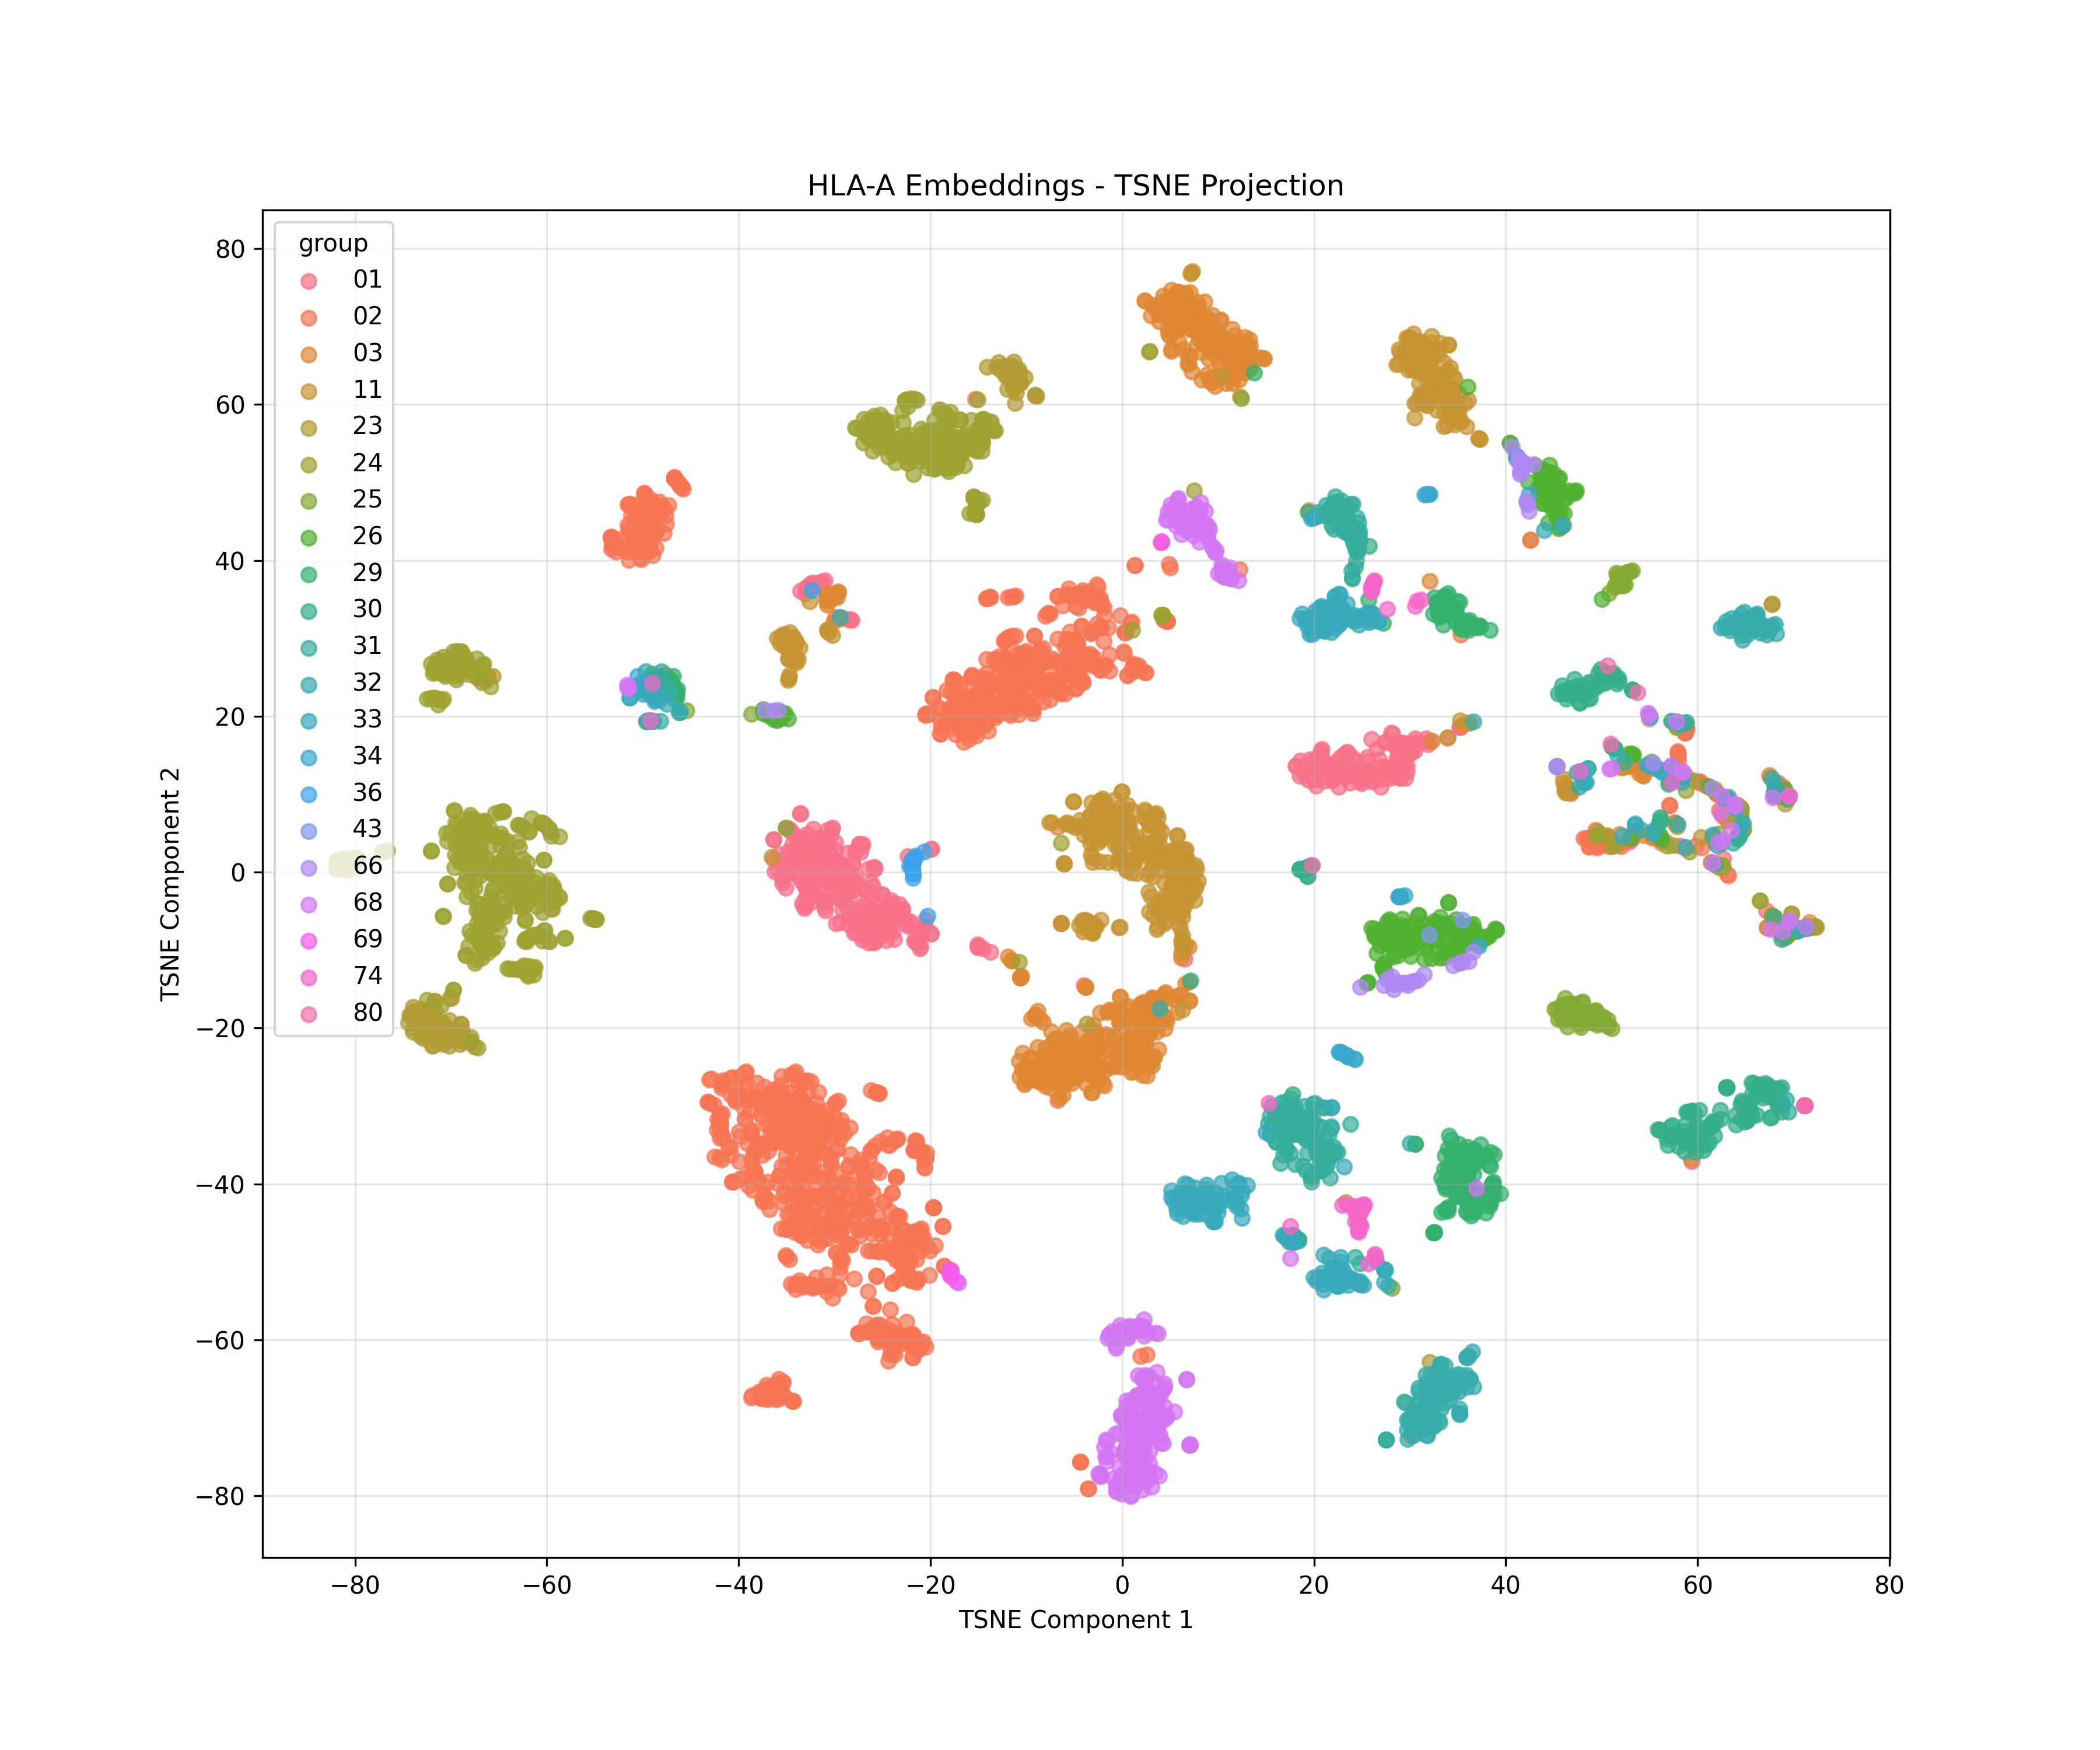
\includegraphics[width=0.32\textwidth]{data/analysis/locus_embeddings/class1/plots/hla_A_tsne.png}
    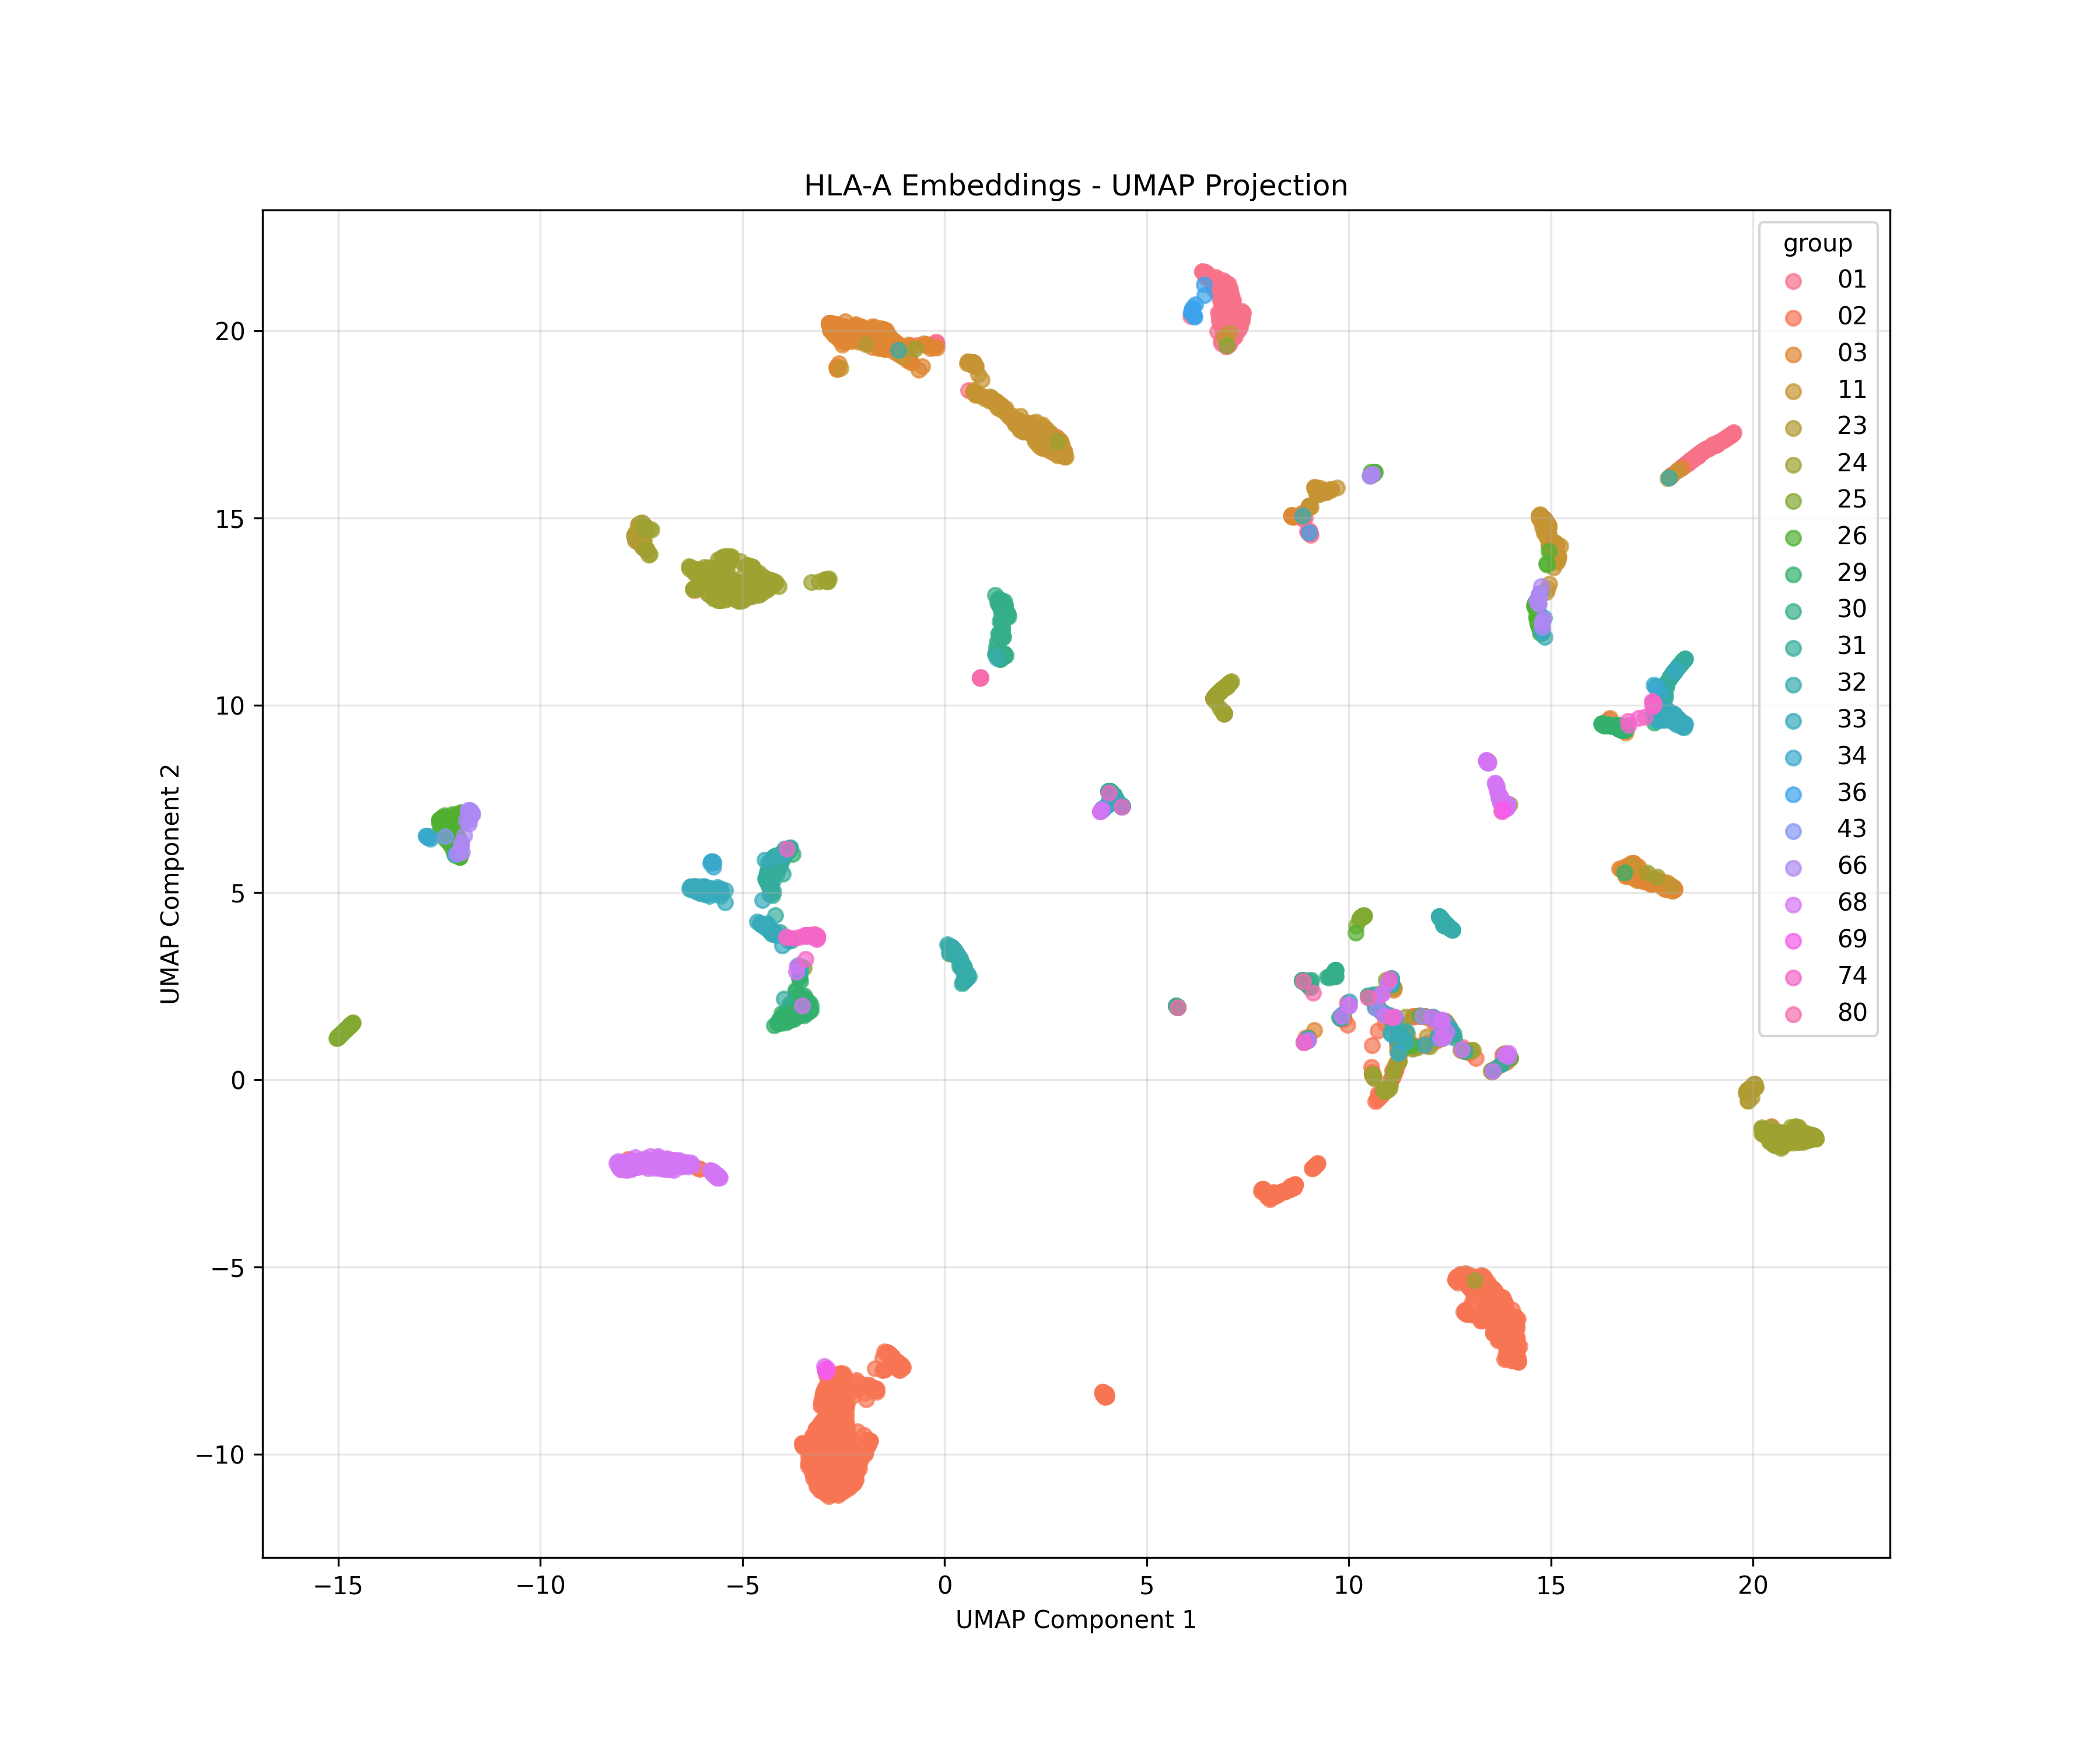
\includegraphics[width=0.32\textwidth]{data/analysis/locus_embeddings/class1/plots/hla_A_umap.png}
    \caption{\small PCA (left), t-SNE (middle), UMAP (right)}
  \end{figure}
  
  \begin{columns}
    \begin{column}{0.5\textwidth}
      \begin{tcolorbox}[colback=gray!5,colframe=gray!40]\small
      \forclinical{Helps identify potential cross-reactive epitopes}
      \end{tcolorbox}
    \end{column}
    \begin{column}{0.5\textwidth}
      \begin{tcolorbox}[colback=gray!5,colframe=gray!40]\small
      \forbioinformatics{Different methods reveal different relationship aspects}
      \end{tcolorbox}
    \end{column}
  \end{columns}
\end{frame}

\begin{frame}{HLA-B: Most Diverse}
  \begin{center}
    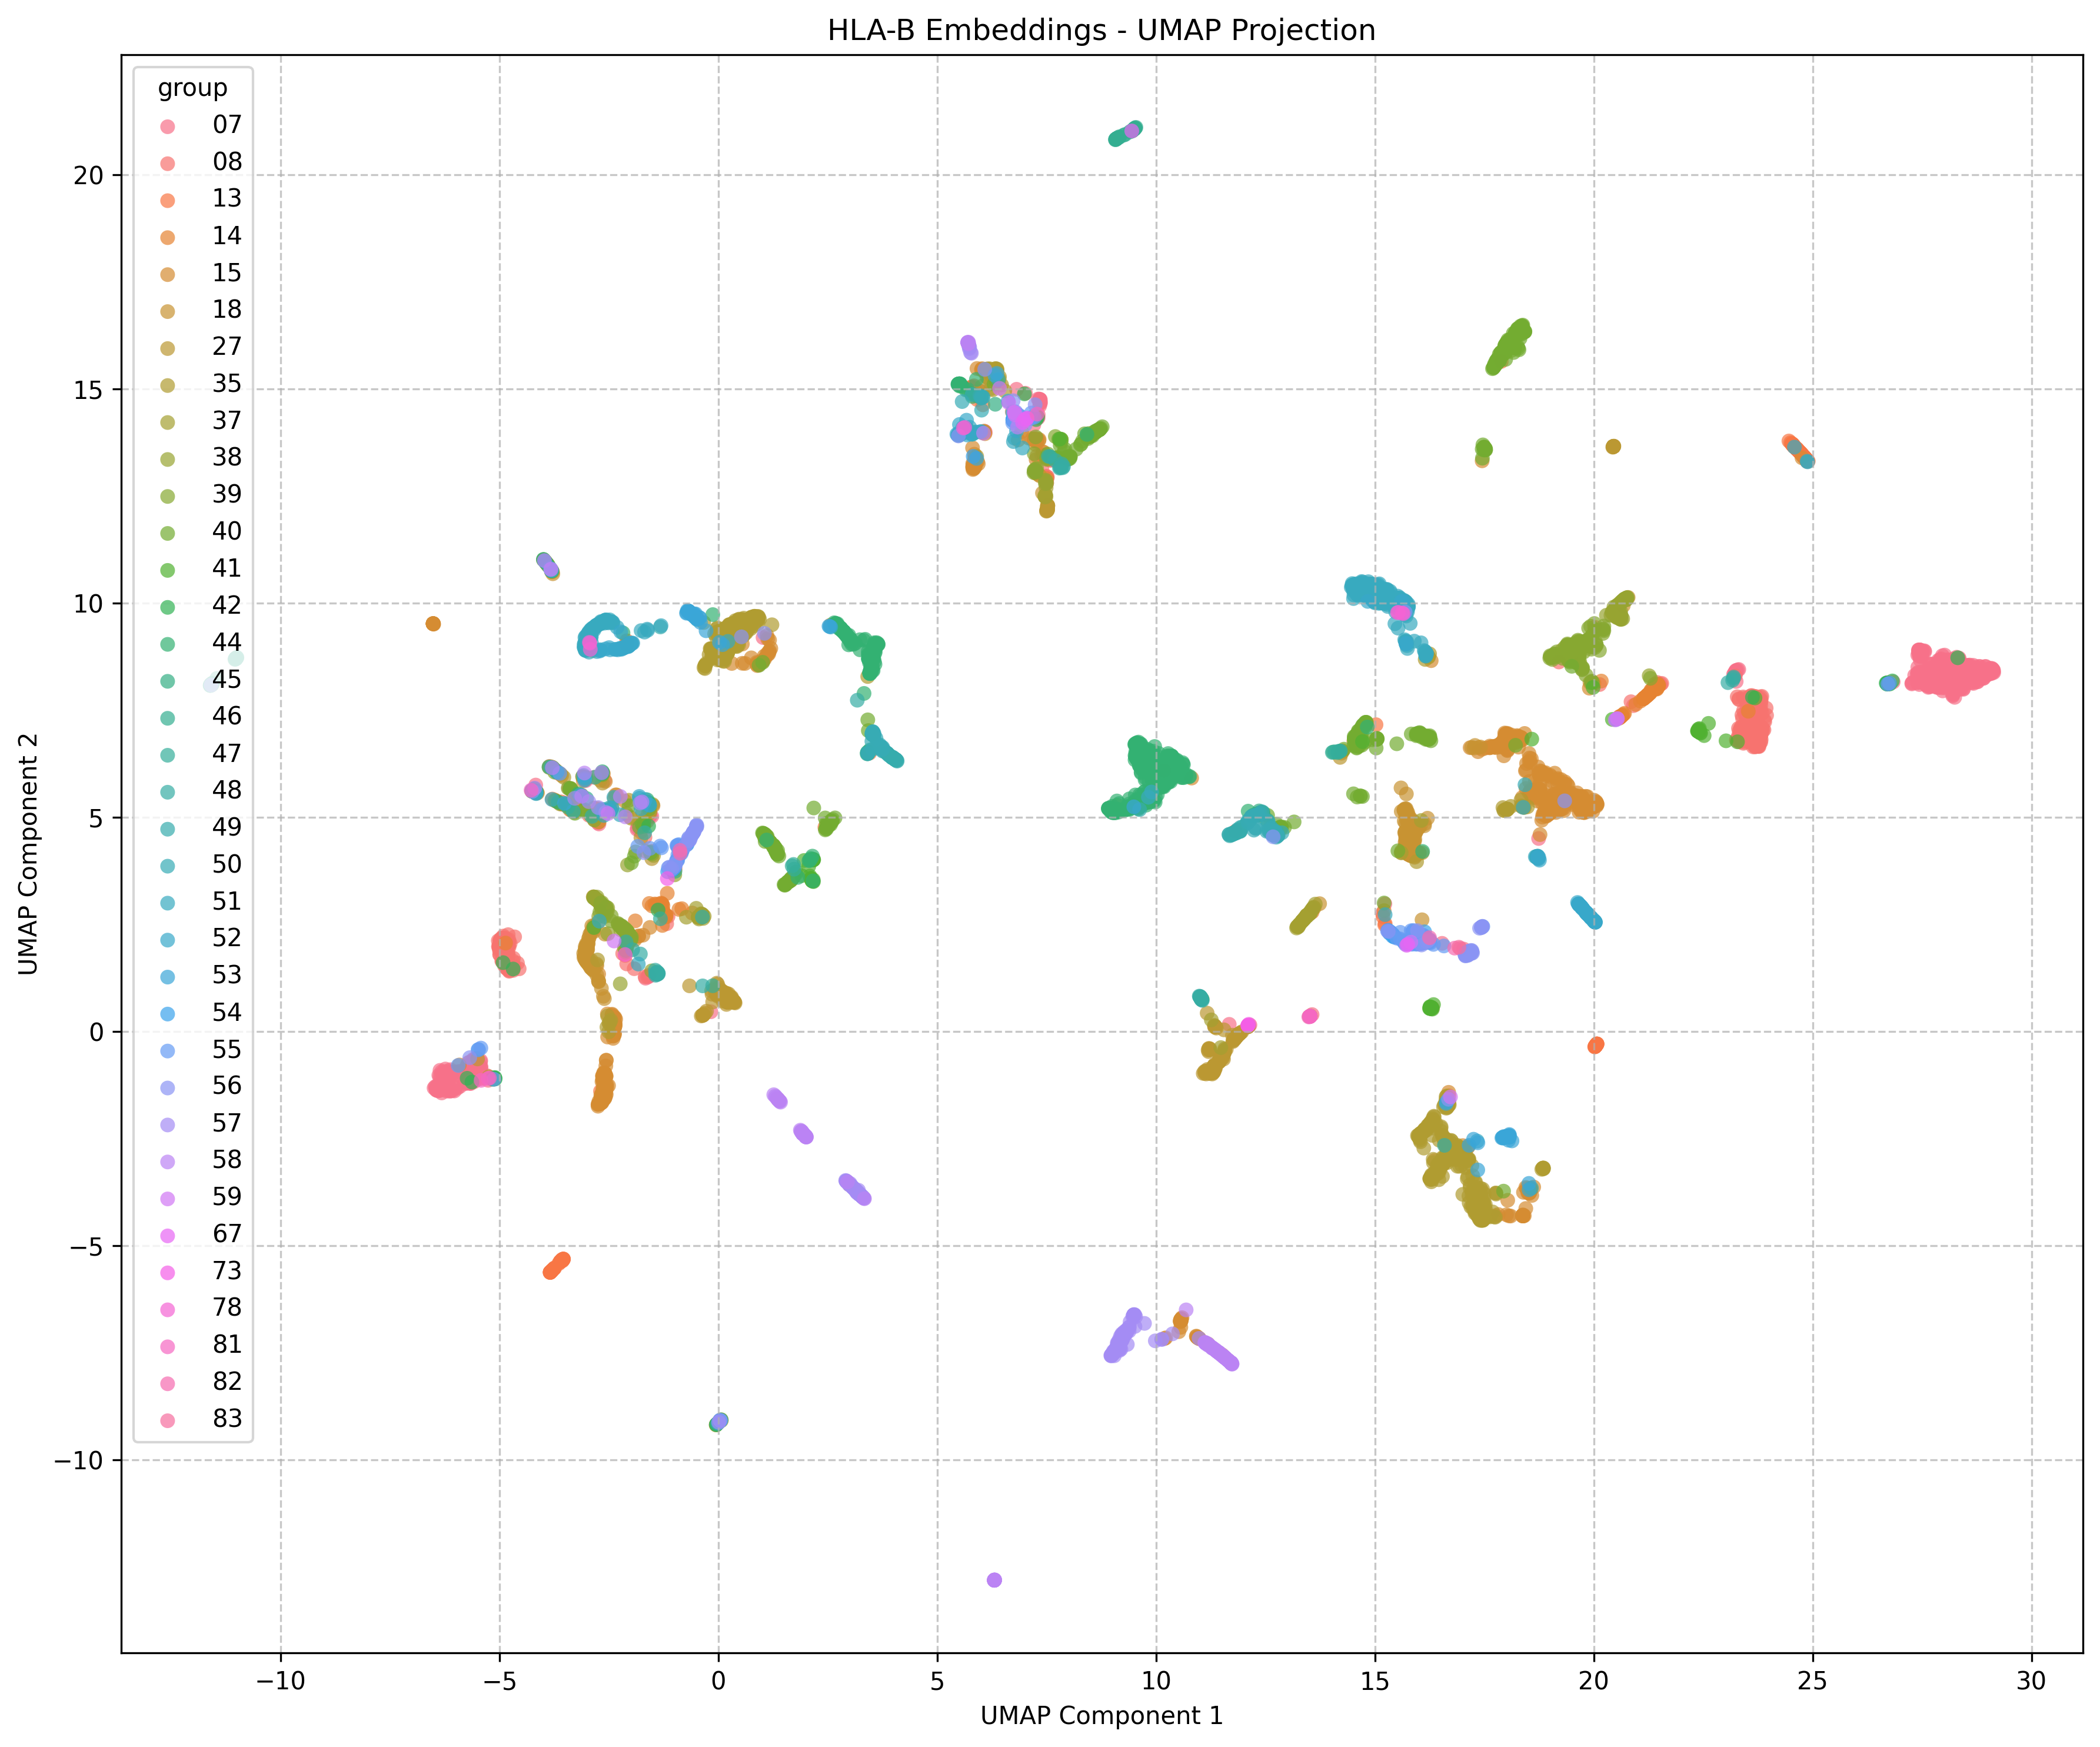
\includegraphics[width=0.5\textwidth]{data/analysis/locus_embeddings/class1/plots/hla_B_umap.png}
  \end{center}
  
  \begin{itemize}\small
    \item Most diverse locus (6,526 alleles)
    \item Complex clustering reflects greater polymorphism
    \item Functional similarity appears more important than sequence
  \end{itemize}
\end{frame}

\begin{frame}{HLA-C: Distinct Patterns}
  \begin{center}
    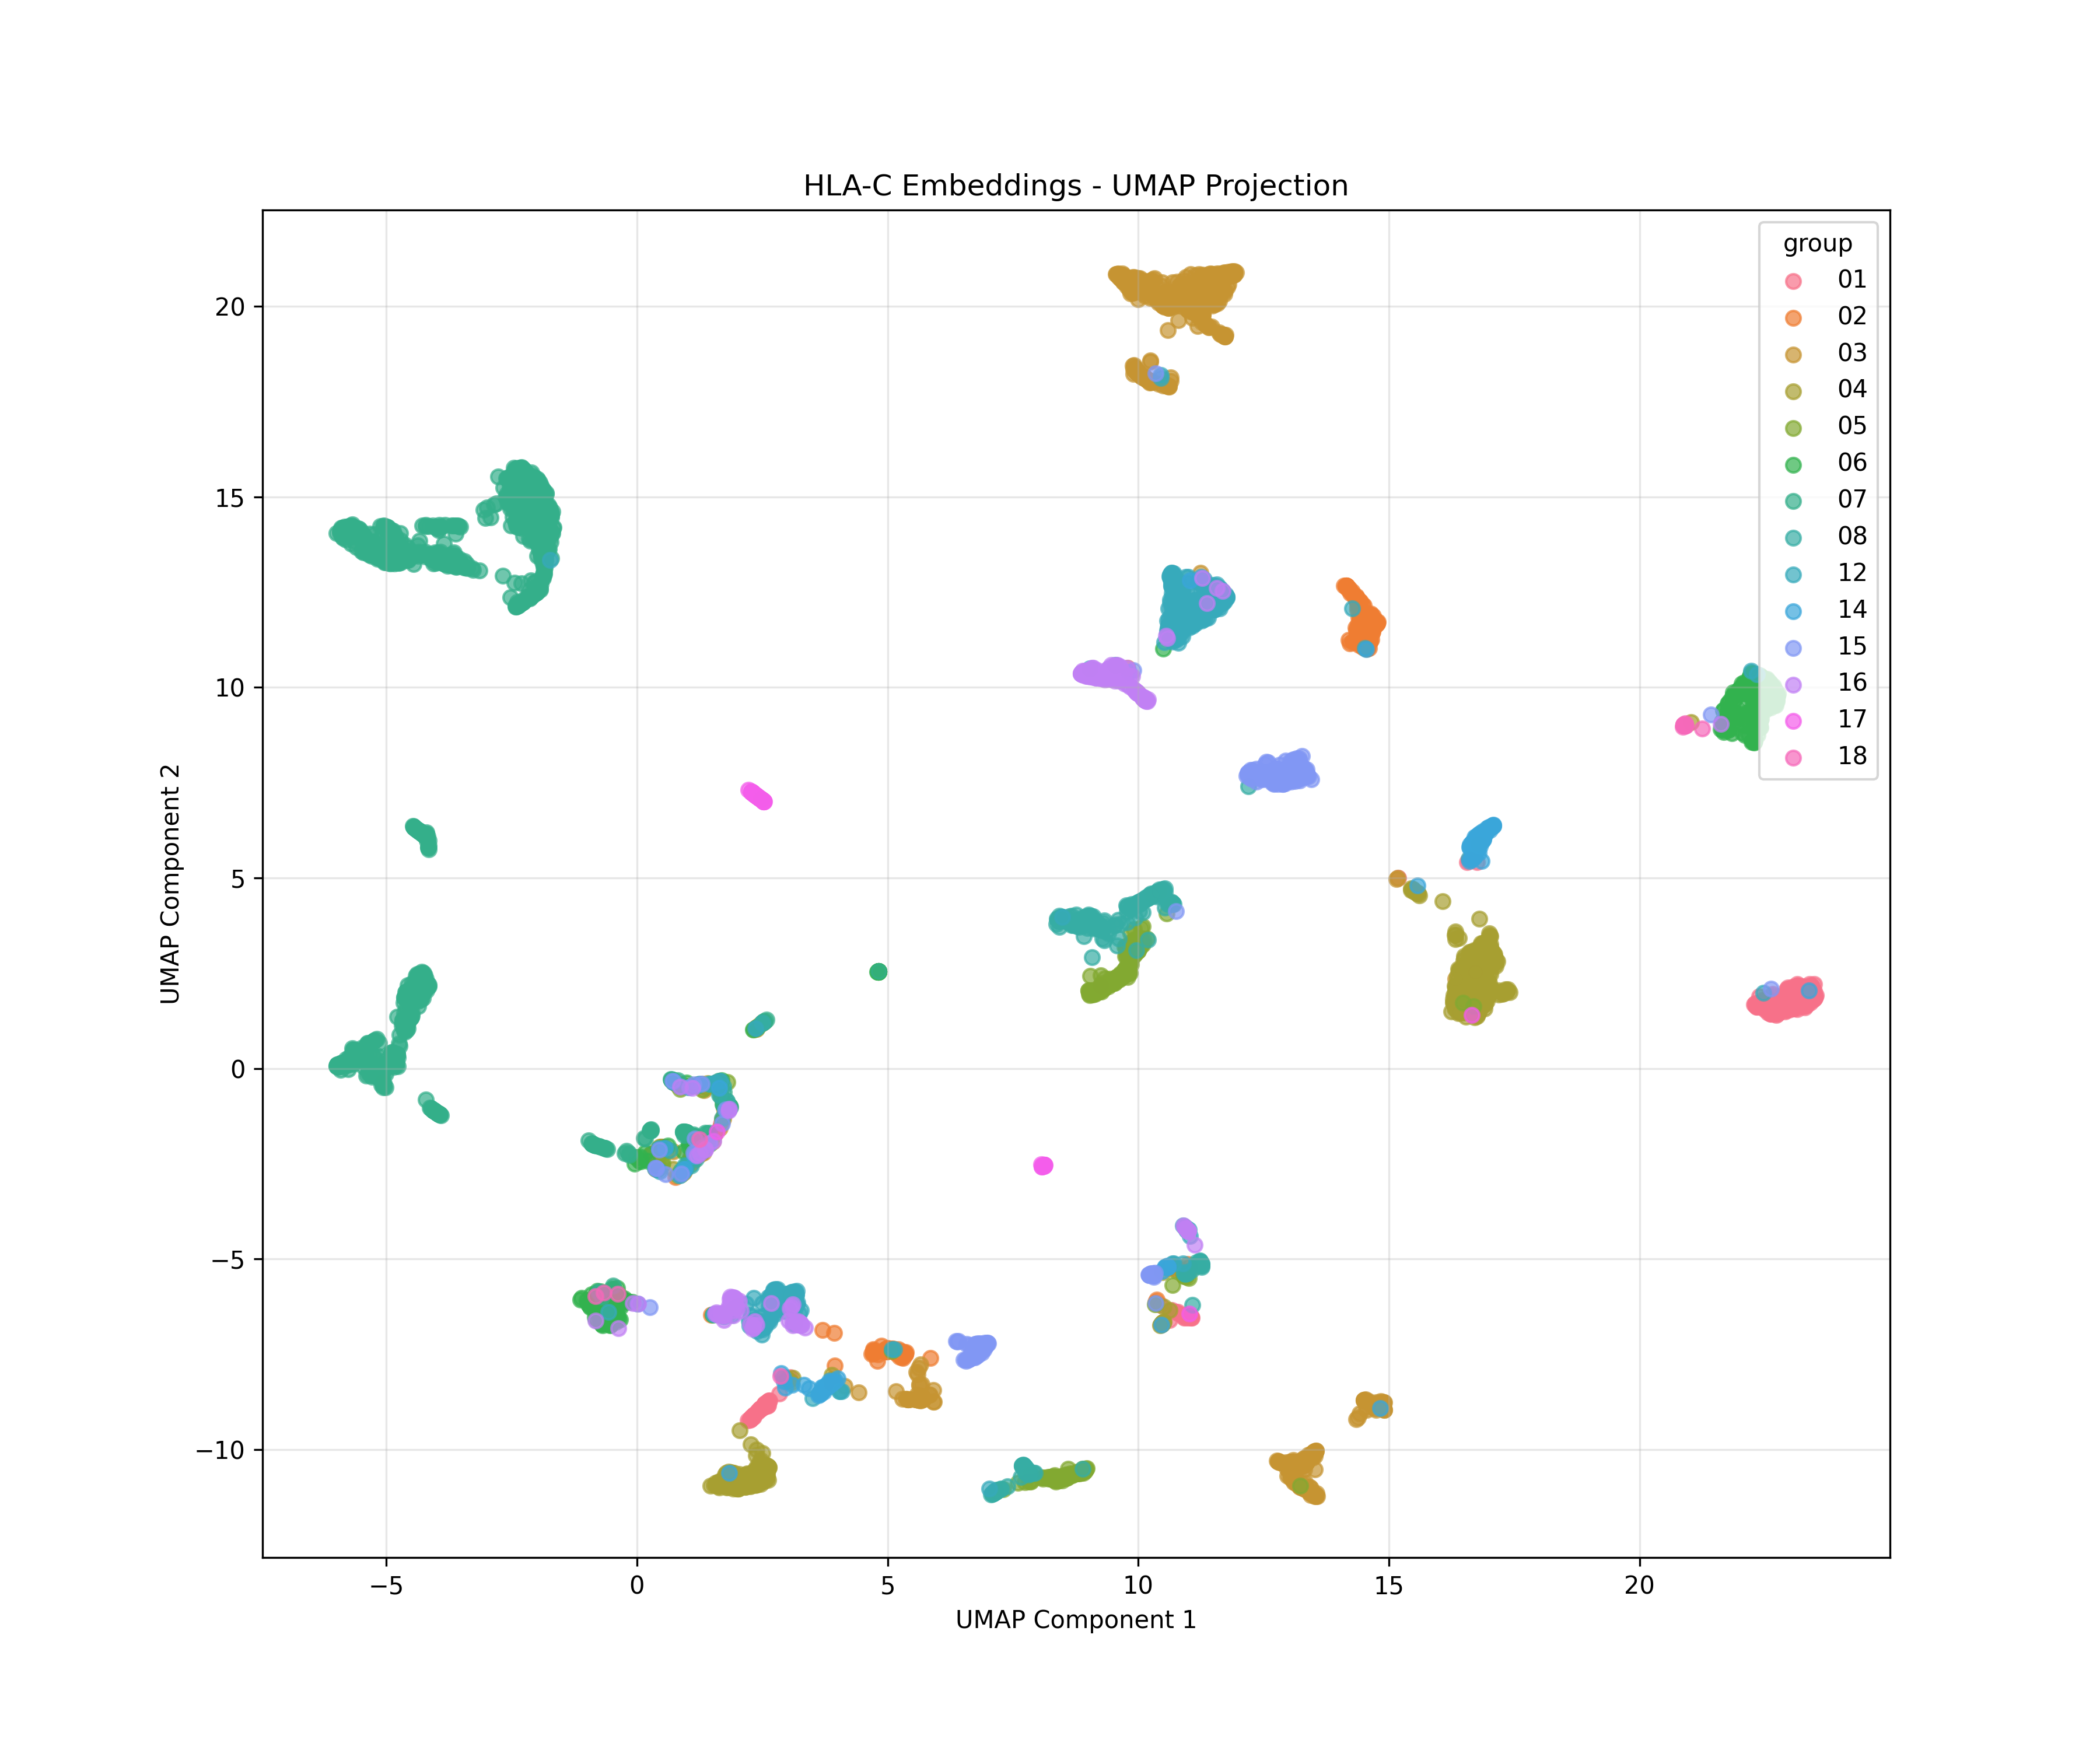
\includegraphics[width=0.5\textwidth]{data/analysis/locus_embeddings/class1/plots/hla_C_umap.png}
  \end{center}
  
  \begin{itemize}\small
    \item More compact clusters than A and B loci
    \item Clearer separation between major groups
    \item Patterns reflect NK cell regulation function
  \end{itemize}
\end{frame}

\section{Applications}

\begin{frame}{Current Applications}
  \begin{columns}
    \begin{column}{0.5\textwidth}
      \textbf{Clinical}
      \begin{itemize}\small
        \item \forclinical{Better matching prediction}
        \item \forclinical{Novel allele classification}
        \item \forclinical{Cross-reactivity assessment}
      \end{itemize}
    \end{column}
    \begin{column}{0.5\textwidth}
      \textbf{Research \& Technical}
      \begin{itemize}\small
        \item \forbioinformatics{Structure-function modeling}
        \item \formanagement{Efficient analysis workflow}
        \item \forbioinformatics{Evolutionary analysis}
      \end{itemize}
    \end{column}
  \end{columns}
  
  \begin{tcolorbox}[colback=hlablue!5,colframe=hlablue]\small
  Understanding functional relationships between HLA alleles has direct applications in transplantation, disease association, and drug response prediction.
  \end{tcolorbox}
\end{frame}

\begin{frame}{Future Directions}
  \begin{columns}
    \begin{column}{0.5\textwidth}
      \textbf{Technical Advancements}
      \begin{itemize}\small
        \item HLA-specific training
        \item Structural information integration
        \item Multi-modal models
      \end{itemize}
      
      \textbf{Data Integration}
      \begin{itemize}\small
        \item Clinical outcome correlation
        \item Population genetics
        \item Cross-species analysis
      \end{itemize}
    \end{column}
    \begin{column}{0.5\textwidth}
      \textbf{Potential Impact}
      \begin{itemize}\small
        \item \forclinical{Improved virtual crossmatching}
        \item \formanagement{Better matching algorithms}
        \item \forbioinformatics{Novel evolutionary insights}
      \end{itemize}
    \end{column}
  \end{columns}
\end{frame}

\begin{frame}{Key Takeaways}
  \begin{tcolorbox}[colback=white,colframe=hlablue!75!black]
  \begin{enumerate}\small
    \item AI embeddings reveal functional HLA relationships
    \item 17,109 alleles analyzed in 81.57 seconds
    \item Clear functional clustering observed
    \item Multiple visualization techniques provide complementary views
    \item Applications span clinical, research, and data domains
  \end{enumerate}
  \end{tcolorbox}
  
  \begin{columns}
    \begin{column}{0.33\textwidth}
      \begin{tcolorbox}[colback=gray!5,colframe=gray!40]\small
      \forclinical{Explore matching prediction applications}
      \end{tcolorbox}
    \end{column}
    \begin{column}{0.33\textwidth}
      \begin{tcolorbox}[colback=gray!5,colframe=gray!40]\small
      \formanagement{Consider workflow integration}
      \end{tcolorbox}
    \end{column}
    \begin{column}{0.33\textwidth}
      \begin{tcolorbox}[colback=gray!5,colframe=gray!40]\small
      \forbioinformatics{Explore additional models}
      \end{tcolorbox}
    \end{column}
  \end{columns}
\end{frame}

\begin{frame}[allowframebreaks]{References}
  \bibliography{references}
\end{frame}

% Technical Appendix
\appendix
\section{Technical Appendix}

\begin{frame}{Technical Details}
  \begin{columns}
    \begin{column}{0.5\textwidth}
      \textbf{Model Specifications}
      \begin{itemize}\small
        \item 30 transformer layers 
        \item 16 attention heads
        \item 1024-dimensional embeddings
        \item 16M parameters (vs. billions)
        \item Pre-trained on 106M proteins
      \end{itemize}
    \end{column}
    \begin{column}{0.5\textwidth}
      \textbf{Implementation}
      \begin{itemize}\small
        \item Hugging Face Transformers
        \item CUDA GPU acceleration
        \item Embedding caching
        \item Batch processing (batch\_size=8)
      \end{itemize}
    \end{column}
  \end{columns}
  
  \textbf{Dimensionality Reduction Parameters}
  \begin{itemize}\small
    \item \textbf{UMAP:} n\_neighbors=15, min\_dist=0.1
    \item \textbf{t-SNE:} perplexity=30, learning\_rate=200
    \item \textbf{PCA:} n\_components=2
  \end{itemize}
\end{frame}

\end{document}
